
\documentclass{article} % Don't change this

\usepackage{tabularx} % extra features for tabular environment
\usepackage{amsmath}  % improve math presentation
\usepackage{graphicx} % takes care of graphic including machinery
\usepackage[margin=1.25in,letterpaper]{geometry} % decreases margins
\usepackage{cite} % takes care of citations
\usepackage{subfigure}
\usepackage{float}    % For tables and other floats
\usepackage[final]{hyperref} % adds hyper links inside the generated pdf file
\usepackage{listings}
\usepackage[framed,numbered,autolinebreaks,useliterate]{mcode}
\usepackage{lipsum}
\usepackage{appendix}
\usepackage{cite}
\hypersetup{
	colorlinks=true,       % false: boxed links; true: colored links
	linkcolor=blue,        % color of internal links
	citecolor=blue,        % color of links to bibliography
	filecolor=magenta,     % color of file links
	urlcolor=blue         
}
\newcommand{\blah}{blah blah blah \dots}



\setlength{\marginparwidth}{3.4cm}

% NEW COUNTERS
\newcounter{points}
\setcounter{points}{100}
\newcounter{spelling}
\newcounter{usage}
\newcounter{units}
\newcounter{other}
\newcounter{source}
\newcounter{concept}
\newcounter{missing}
\newcounter{math}

% COMMANDS
%\newcommand{\raisa}[2]{\colorbox{Yellow}{#1} \todo{#2}}
\newcommand{\arbitrary}[2]{\todo{#1 #2} \addtocounter{points}{#2} \addtocounter{other}{#2}}
\newcommand{\english}{\todo{LANGUAGE (-1)} \addtocounter{points}{-1}
\addtocounter{usage}{-1}}
\newcommand{\units}{\todo{UNITS (-1)} \addtocounter{points}{-1}
\addtocounter{units}{-1}}
\newcommand{\spelling}{\todo{SPELLING and GRAMMAR (-1)} \addtocounter{points}{-1}
\addtocounter{spelling}{-1}}
\newcommand{\source}{\todo{SOURCE(S) (-2)} \addtocounter{points}{-2}
\addtocounter{source}{-2}}
\newcommand{\concept}{\todo{CONCEPT (-2)} \addtocounter{points}{-2}
\addtocounter{concept}{-2}}
\newcommand{\missing}[2]{\todo{MISSING CONTENT (#1) #2} \addtocounter{points}{#1}
\addtocounter{missing}{#1}}
\newcommand{\maths}{\todo{MATH (-1)} \addtocounter{points}{-1}
\addtocounter{math}{-1}}

\newcommand{\summary}[1]{
\begin{mdframed}[nobreak=true]
\begin{minipage}{\textwidth}
\vspace{0.5cm}
\begin{center}
\Large{Grade Summary} \hrule 
\end{center} \vspace{0.5cm}
General Comments: #1

\vspace{0.5cm}
Possible Points \dotfill 100 \\
Points Lost (Spelling and Grammar) \dotfill \thespelling \\
Points Lost (Language) \dotfill \theusage \\
Points Lost (Units) \dotfill \theunits \\
Points Lost (Math) \dotfill \themath \\
Points Lost (Sources) \dotfill \thesource \\
Points Lost (Concept) \dotfill \theconcept \\
Points Lost (Missing Content) \dotfill \themissing \\
Other \dotfill \theother \\[0.5cm]
\begin{center}
\large{\textbf{Grade:} \fbox{\thepoints}}
\end{center}
\end{minipage}
\end{mdframed}}

%#########################################################

%To use symbols for footnotes
\renewcommand*{\thefootnote}{\fnsymbol{footnote}}
%To change footnotes back to numbers uncomment the following line
%\renewcommand*{\thefootnote}{\arabic{footnote}}

% Enable this command to adjust line spacing for inline math equations.
% \everymath{\displaystyle}

% _______ _____ _______ _      ______ 
%|__   __|_   _|__   __| |    |  ____|
%   | |    | |    | |  | |    | |__   
%   | |    | |    | |  | |    |  __|  
%   | |   _| |_   | |  | |____| |____ 
%   |_|  |_____|  |_|  |______|______|
%%%%%%%%%%%%%%%%%%%%%%%%%%%%%%%%%%%%%%%

\title{
\normalfont \normalsize 
\textsc{Rutgers University \\ 
Summer Research Program} \\
[10pt] 
\rule{\linewidth}{0.5pt} \\[6pt] 
\huge Preparation for GpyTorch Implementation  \\
\rule{\linewidth}{2pt}  \\[10pt]
}
\author{Han Liu}
\date{\normalsize \today}

\begin{document}

\maketitle



\section{Introduction}
In this week, I have read the second paper "Exact Gaussian Processes on a Million Data Points" and have finished all the preparation work for the final GpyTorch Implementation by Matlab. Specifically, firstly I have fixed the error of Pivoting Cholesky Decomposition, and try to implement it with Matlab. Secondly, I use the result of Pivoting Cholesky Decomposition as a preconditioner to the conjugate gradient algorithm, the result shows the preconditioning accelerate the convergence significantly. Thirdly, I have figured out the Stochastic Trace Estimation, and the MATLAB results shows the fast convergence of the algorithm with the increasing of sampling times. Finally, I have figured out the innovative algorithm proposed by the second paper.\\

\noindent In the following week, I will implement the whole Gaussian Process (GP) using GPU acceleration algorithm proposed by this paper, and I will use Adam optimizer to train GP, on which I am currently working.


\section{The Pivoting Cholesky Decomposition}
In the process of implementing the pivoting cholesky decomposition (PCC), I found the algorithm I derived last week had some problems, so I have implemented it again. Specifically, we need to find $P^TKP=R^TR$ for symmetric positive matrix $K\in R^{n\times n}$, where $P$ is permutation matrix. Following the derivation of the pivoting cholesky decomposition in the paper, we need to use one propertiy of permutation matrix:
\begin{equation}
P^{-1}=P^{T}
\end{equation}
The mathematical details are given in appendix. Specifically, the whole algorithm should be as following \cite{1}:
 \begin{figure}[h]
	\begin{center}
		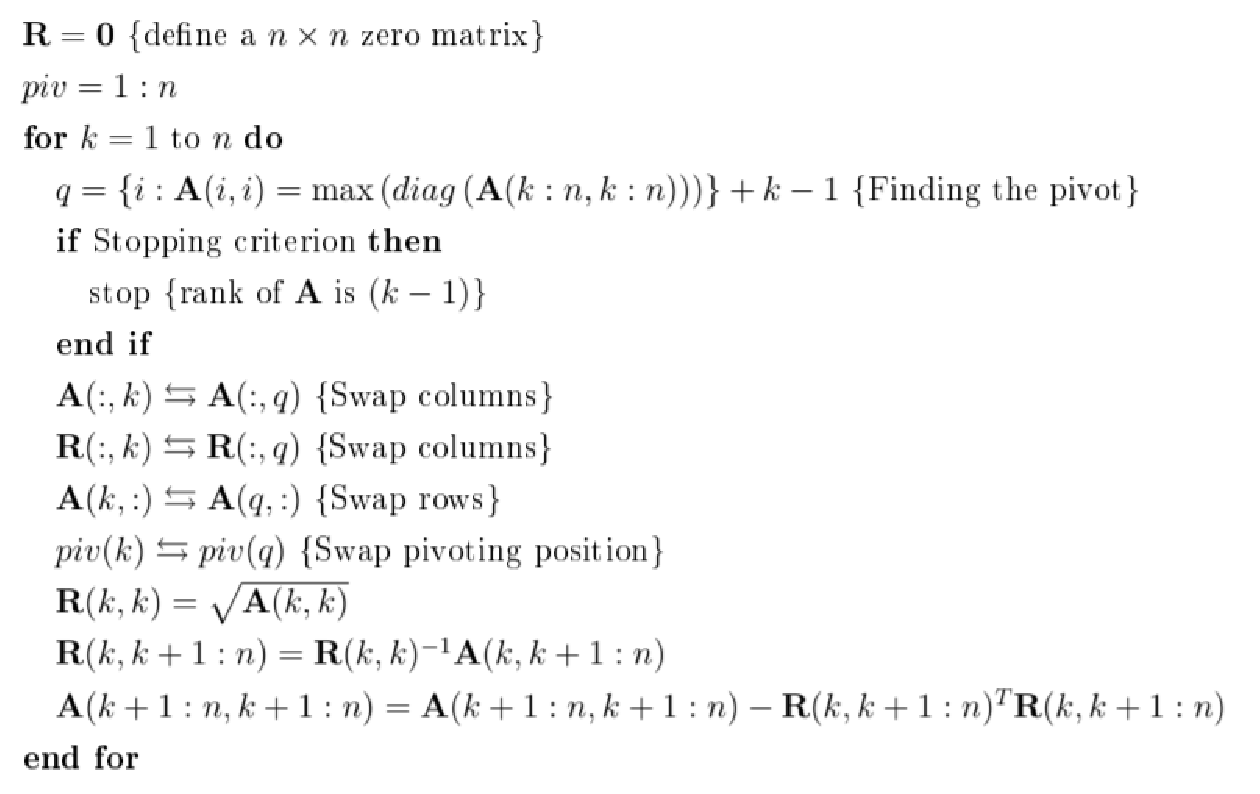
\includegraphics[width=0.7\textwidth]{PCC}
	\end{center}
	\caption{Pseudo-code for Pivoting Cholesky Decomposition}
	\label{fig1}
\end{figure}
We use a random matrix $D$ to be the matrix waiting for decomposition, and a simple provement can be seen as following:
 \begin{figure}[h]
	\begin{center}
		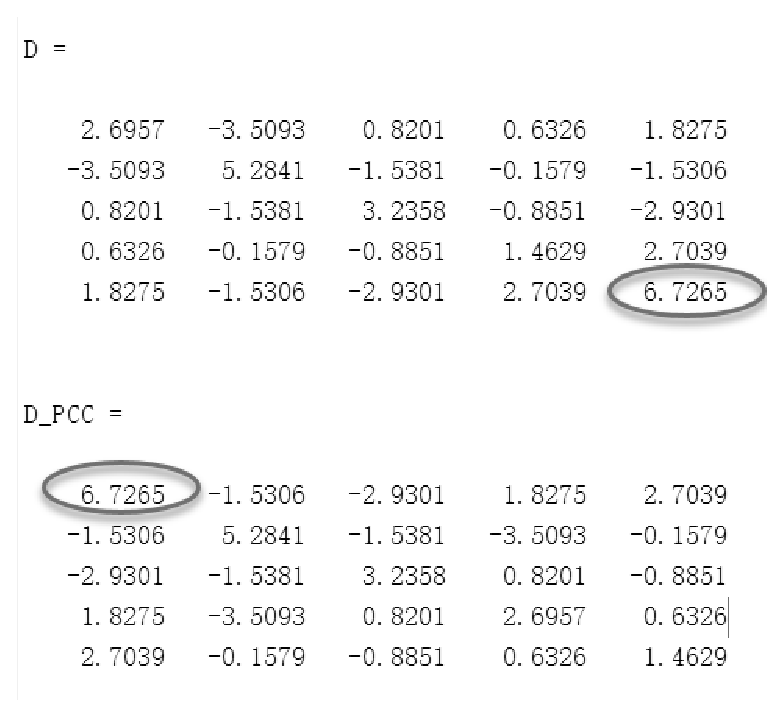
\includegraphics[width=0.4\textwidth]{test1}
	\end{center}
	\caption{Pseudo-code for Pivoting Cholesky Decomposition}
	\label{fig2}
\end{figure}
The maximum diagonal element of original matrix is at the bottom right corner, after the decomposition, the reconstructed result is exchanged to the top left corner, and after exchanging the pivoting row and column of original matrix, they are the same.\\
The main objective of using PCC is to use it as a preconditioner for conjugate gradient algorithm (CG). In this process, we need to satisfy:
\begin{equation}\label{eq2}
(M+\sigma ^2I)^{-1}\hat{K}\approx I
\end{equation}
Where $M$ is the result of PCC of $K$, $\hat{K}=K+\sigma ^2I$. In order to satisfy the requirement of Eq. \ref{eq2}, we need to rearrange the results of PCC, this can be done by:
\begin{equation}
K=(P^T)^{-1}R^TRP^{-1}=PR^TRP^T
\end{equation}
The Matlab code is as following:
\begin{lstlisting}
%Implementation of Pivoted Cholesky Composition
function [ G ] = Pivited_Cholesky_Composition( A )
n=size(A,1);
v=randperm(n);
Pi = sort(v);
l=zeros(n,n);   %triangular matrix we want 
P=zeros(n,n);
for k=1:n
[~, p]=max(diag(A(k:n,k:n)));
i=p+k-1;

a=A(:,k);   %exchange column
A(:,k)= A(:,i);
A(:,i)=a;

b=l(:,k);       %exchange L
l(:,k)=l(:,i);
l(:,i)=b;

c=A(k,:);       %exchange row
A(k,:)=A(i,:);
A(i,:)=c;

a=Pi(k);        %exchange pi
Pi(k)=Pi(i);
Pi(i)=a;

l(k,k)=sqrt(A(k,k));
l(k,k+1:n)=l(k,k)\A(k,k+1:n);
A(k+1:n,k+1:n)=A(k+1:n,k+1:n)-l(k,k+1:n)'*l(k,k+1:n);
P(Pi(k),k)=1;
end
Am=l'*l;
%exchange back the pivoted position
G=P*Am*P';
\end{lstlisting}

\section{Preconditioning}
The basic idea of preconditioning is to introduce a matrix $P$ to solve the linear system:
\begin{equation}
P^{-1}\hat{K}u=P^{-1}y
\end{equation} 
The preconditioning will guarantee to have the same solution with the original linear system, and the system's convergence is depend on the conditioning of $P^{-1}\hat{K}$ rather than $\hat{K}$. Furthermore, if $P^{-1}\hat{K}\approx I$, the system will converge fastly, thus we will use the decomposition result of PCC as preconditioner. As for the implementation of preconditioned conjugate gradients (PCG), there are some mistakes of the pseudo-code given in the paper, the correct version is given as following:
 \begin{figure}[H]
	\begin{center}
		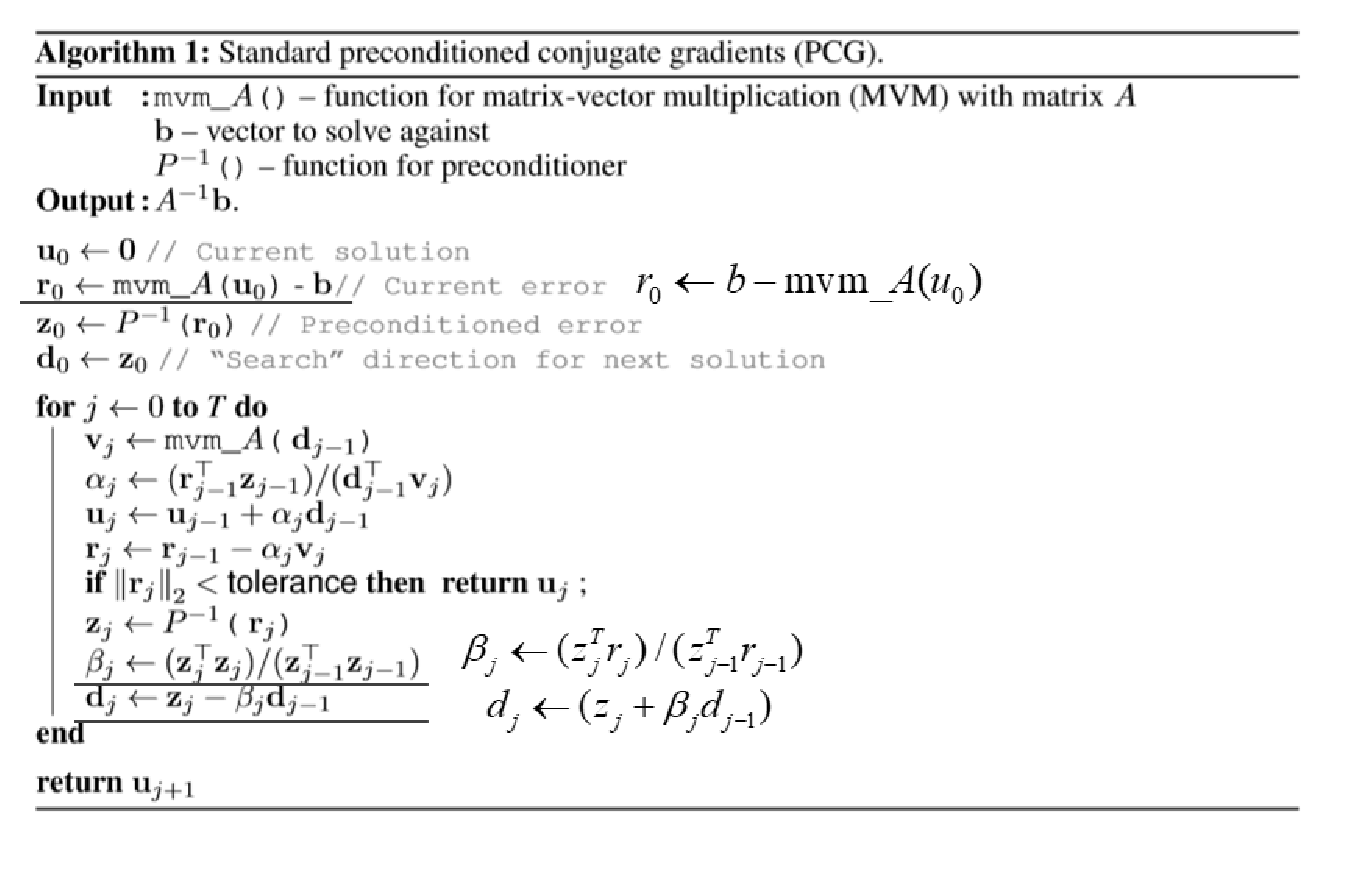
\includegraphics[width=0.65\textwidth]{PCG}
	\end{center}
	\caption{Algorithm of Preconditioned Conjugate Gradients}
	\label{fig3}
\end{figure}
I have also compared the results of Non-preconditioning PCG with Preconditioning PCG, their results are as following: 

\begin{figure}[H]
	\centering
	\subfigure[Non-preconditioning]{\includegraphics[width=2.7in]{non-err}}
	\subfigure[Preconditioning]{\includegraphics[width=2.7in]{pre-err}}
	\caption{Comparison of Two Implementations}
	\label{fig4}
\end{figure}
The results show the preconditioning accelerates the speed of convergence significantly. The Matlab code is as following:
\begin{lstlisting}
%Standard preconditioned conjugate gradients
function [ c ] = Standard_PCG( mvm_A,b, M )
n=size(mvm_A,1);
T=50;        %number of iteration
e=0.0001;   %tolerance


%initialization
u=zeros(n,T);
r=zeros(n,T);
z=zeros(n,T);
d=zeros(n,T);
v=zeros(n,T);
alpha=zeros(1,T);
beta=zeros(1,T);
truth=inv(mvm_A)*b;

%main program
r(:,1)=b-mvm_A*u(:,1);          %error fixed
z(:,1)=M*r(:,1);            %changes to PCG
d(:,1)=z(:,1);
E=zeros(1,T);

for j=2:T
v(:,j)=mvm_A*d(:,j-1);
alpha(j)=(z(:,j-1)'*r(:,j-1))./(d(:,j-1)'*v(:,j));
u(:,j)=u(:,j-1)+alpha(j)*d(:,j-1);
r(:,j)=r(:,j-1)-alpha(j)*v(:,j);
if norm(r(:,j),2)<e
break
end
z(:,j)=M*r(:,j);        %changes to PCG
beta(j)=(z(:,j)'*r(:,j))./(z(:,j-1)'*r(:,j-1));     %error fixed
d(:,j)=z(:,j)+beta(j)*d(:,j-1);                 %error fixed
E(j)=norm(truth-u(:,j),1);
end
E(1)=E(2);
n=1:T;
figure(1);
plot(n,E);xlabel('N');ylabel('Error');title('Error of Preconditioned PCG during each iteration time');
c=E;
\end{lstlisting}

\section{Stochastic Trace Estimation}
Stochastic Trace Estimation (STE) \cite{2} is useful when determining $log|\hat{K}|$, $tr(\hat{K}^{-1}\frac{\partial \hat{K}}{\partial \theta})$, specifically, we have:
\begin{equation}
Tr(\hat{K}^{-1}\frac{\partial \hat{K}}{\partial \theta})=E[z_i^T\hat{K}^{-1}\frac{\partial \hat{K}}{\partial \theta}z_i]
\end{equation}
\begin{equation}
log|\hat{K}|=Tr(logT)=E[z_i^T(logT)z_i]
\end{equation}
Where the mean can be estimated by arithmetic mean:
\begin{equation}
E[z_i^T(logT)z_i]=\frac{1}{N}\sum_{i=1}^{N}z_i^T(logT)z_i
\end{equation}
The arithmetic mean converges to the mean with the increasing of N, which can be illustrated by the following graph:
 \begin{figure}[H]
	\begin{center}
		\includegraphics[width=0.65\textwidth]{error}
	\end{center}
	\caption{Convergence of Stochastic Trace Estimation}
	\label{fig5}
\end{figure}
 
 \section{Partitioned kernel MVMs}
 The second paper (Exact Gaussian Processes on a Million Data Points) propose a new intuitive method of calculating MVM. In the process of PCG, the  computation which takes the most memory usage is $v=\hat{K}*d$, which is costs $O(n^2)$ memory. We can divide data matrix $X$ into $p$ partitions:
 \begin{equation}
 X=[X^{(1)};...;X^{(p)}]
 \end{equation} 
 where we use “ ;” to denote row-wise concatenation. Then the kernel matrix can be concatenated as:
 \begin{equation}
 \hat{K}=[\hat{K}_{X^{(1)}X};...;\hat{K}_{X^{(p)}X}]
 \end{equation}
 Then we can rewrite the matrix-vector product $\hat{K}v$ as:
 \begin{equation}
 \hat{K}v=[\hat{K}_{X^{(1)}X}v;...;\hat{K}_{X^{(p)}X}v]
 \end{equation}
 This process is very intuitive, when the iteration time $p\rightarrow n$, the PCG only needs $O(n)$ memory.
\begin{thebibliography}{1}
	\bibitem{1}L. S. Bastos, A. O. Hagan, "Pivoting Cholesky Decomposition applied to Emulation", June, 2007.
	\bibitem{2}Fika, Paraskevi, and Christos Koukouvinos. "Stochastic estimates for the trace of functions of matrices via Hadamard matrices." Communications in Statistics-Simulation and Computation 46.5 (2017): 3491-3503.
	
	
\end{thebibliography}


\begin{appendices}
	\section{Derivation of PCD}
	 \begin{figure}[H]
		\begin{center}
			\includegraphics[width=0.65\textwidth]{111}
		\end{center}
		\caption{Derivation of PCD}
		\label{fig7}
	\end{figure}

\end{appendices}


\end{document} % NOTHING AFTER THIS LINE IS PART OF THE DOCUMENT
